\section{From classical to relativistic quantum mechanics}\label{sec:FromClassicalToRelativisticQM}
Classical mechanics is based on the quantization of classical observable by promoting them to operators, with their own commutation relations. De Broglie suggested that every quantum object can be described in terms of waves proprieties related to the energy and the momentum of the object:
\begin{equation*}
    E=h\nu,\ \vec p=h\vec k,\qquad \Rightarrow\qquad \psi(\vec x,t)=\exp\biggl(\frac{i}{\hslash}P^\mu x_\mu\biggr),\quad P^\mu=\bigg(\frac{E}{c},\vec p\bigg).
\end{equation*}
Schrödinger was the first to propose this quantization procedure in order to find the equation of motion of these objects: in a simpler way than what he did, we can observe that the differentiation operators applied to $\psi$ act as operators with eigenvalues related to the components of $P^\mu$.
\begin{equation*}
    i\hslash\frac{\partial}{\partial t}\psi=E\psi=\frac{{\vec p}^2}{2m}\psi=(-i\hslash\vec\nabla)(-i\hslash\vec\nabla)\frac{\psi}{2m}=-\frac{\hslash^2}{2m}{\vec\nabla}^2\psi.
\end{equation*}
In this way we've got the \textbf{Schrödinger equation}. The same approach can be used in order to derive the relativistic equations of motion:
\begin{equation*}
    E=\sqrt{p^2c^2+m^2c^4}\quad\rightarrow\quad i\hslash\frac{\partial}{\partial t}\psi=\sqrt{-\hslash^2c^2\vec\nabla^2+m^2c^4}\psi.
\end{equation*}
The differential equation is hard to solve since it is not so clear what should be the square root of a derivative, to solve this problem we could Taylor expand the square root, but this leads to a non-local theory.\\Klein and Gordon tried a different approach quantizing $E^2=p^2c^2+m^2c^4$:
\begin{equation}\label{KleinGordonEq}
    -\hslash^2\frac{\partial^2}{\partial t^2}\psi=\bigl(-\hslash^2c^2\vec\nabla^2+m^2c^4\bigr)\psi,
\end{equation} 
this is the \textbf{Klein-Gordon equation}.\\
In equation \eqref{KleinGordonEq} it appears a constant term given by $\frac{mc}{\hslash^2}$, this is called the \textbf{reduced Compton wavelength}.\\
Using natural units ($\hslash=c=1$) and defining the box operator $\Box=\partial^\mu\partial_\mu$, equation \eqref{KleinGordonEq} reads:
\begin{equation}\label{KleinGordonNU}
    (\Box-m^2)\psi=0.
\end{equation}

We will now study the proprieties of the solutions of equation \eqref{KleinGordonNU}.\\Using the ansatz $\psi(x^\mu)\propto e^{iA_\mu x^\mu}$ we get:
\begin{align*}
    (-\partial^\nu\partial_\nu+m^2)e^{iA_\mu x^\mu}=(A^\nu A_\nu+m^2)e^{iA_\mu x^\mu}=0.
\end{align*}
Since the exponential is a positive function, in order to be a solution, $A^\mu$ must satisfy the energy-momentum relation of a particle with mass m, and thus it should be $A^\mu=P^\mu$:
\begin{equation}\label{mass-shellCondition}
    P^0=\pm\sqrt{\vec p^2+m^2}\triangleq \pm E_p,
\end{equation} 
which is the so called \textbf{mass-shell condition}.\\This relation gives rise to a strange behavior of the relativistic free particle: since $P^0$ is the energy of the particle, this equation shows that wave functions with \textbf{negative energies} are allowed by the theory. Defining
\begin{equation*}
    \begin{cases}
        \psi^+_{\vec p}(x^\mu)=e^{-iE_pt}e^{i\vec p\cdot \vec x}\\
        \psi^-_{\vec p}(x^\mu)=e^{iE_pt}e^{-i\vec p\cdot \vec x}
    \end{cases}
\end{equation*}
we can get the general solution \eqref{KleinGordonNU} by superposition of these:
\begin{equation}\label{KGSup}
    \psi(x^\mu)=\int\frac{d^3p}{(2\pi)^3}\frac{1}{2E_p}\biggl(a(\vec p)e^{-iE_pt}e^{i\vec p\cdot \vec x}+b^*(\vec p)e^{iE_pt}e^{-i\vec p\cdot \vec x}\biggr).
\end{equation}
We should observe that, since $   \psi^+_{\vec p}(x^\mu)=  (\psi^-_{\vec p}(x^\mu))^*$, the complex conjugate of a wave function given by \eqref{KGSup} is:
\begin{equation*}
    \psi(x^\mu)^*=\int\frac{d^3p}{(2\pi)^3}\frac{1}{2E_p}\biggl(b(\vec p)e^{-iE_pt}e^{i\vec p\cdot \vec x}+a^*(\vec p)e^{iE_pt}e^{-i\vec p\cdot \vec x}\biggr).
\end{equation*}
We will see that the negative energy components should be interpreted as an antiparticle or the same particle going backwards in time.

Lastly, we will see that the probability interpretation of quantum mechanics can fail due to this negative energy states. Multiplying the Klein-Gordon equation \eqref{KleinGordonNU} by $\psi*$ and combining it with its complex conjugate we get the probability conservation law:
\begin{align*}
    \psi^*(\Box-m^2)\psi-\psi(\Box-m^2)\psi^*&=\psi^*\Box\psi-\psi\Box\psi^*\\&=\partial_\mu(\psi^*\partial^\mu\psi-\psi\partial^\mu\psi^*)=2im\partial_\mu J^\mu=0,\\
    J^\mu\triangleq \frac{1}{2im}(\psi^*\partial^\mu\psi-\psi\partial^\mu\psi^*).
\end{align*} 
The component $J^0$ is therefore the probability density, which can became negative for negative energies. The field should be interpreted as an object whose quanta are the particles we observe.\\ This interpretation leads directly to quantum field theory (Part \ref{part:QFT}).
\section{The Yukawa potential}\index{Yukawa potential}
Since we are going to interpret the wave function resulting form the Klein-Gordon equation \eqref{KleinGordonNU} as we interpret the electromagnetic waves that arise from Maxwell's equations, we could try to include some source terms in this theory too.\\
The first attempt we can try is a point source (like a point charge) stationary:
\begin{equation*}
    (\Box-m^2)\psi(x^\mu)=g\delta^3(x^\mu)\qquad\xrightarrow[case]{Stationary}\qquad\big(\vec \nabla^2-m^2\big)\psi(\vec x)=g\delta^3(\vec x).
\end{equation*}
In order to solve this equation let's consider the Fourier transform of a generic solution and the Fourier representation of the Dirac delta function:
\begin{equation*}
    \psi(\vec x)=\int\frac{d^3k}{(2\pi)^3}e^{i\vec k\cdot \vec x } \tilde{\psi}(\vec p),\qquad \delta^3(\vec x)=\int\frac{d^3k}{(2\pi)^3}e^{i\vec k\cdot \vec x }.
\end{equation*}
Plugging these two in the differential equation, and using the linearity of the nabla operator, we get: 
\begin{align*}
    &\big(\vec \nabla^2-m^2\big)\int\frac{d^3k}{(2\pi)^3}e^{i\vec k\cdot \vec x } \tilde{\psi}(\vec k)=g\int\frac{d^3k}{(2\pi)^3}e^{i\vec k\cdot \vec x },\\&\Rightarrow\qquad\int\frac{d^3k}{(2\pi)^3}e^{i\vec k\cdot \vec x }(-k^2-m^2) \tilde{\psi}(\vec k)=g\int\frac{d^3k}{(2\pi)^3}e^{i\vec k\cdot \vec x };\\&\Rightarrow\qquad \tilde{\psi}(\vec k)=\frac{-g}{k^2+m^2}.
\end{align*}
\marginnote{
    \tdplotsetmaincoords{60}{110}
\begin{tikzpicture}[scale=2, tdplot_main_coords]
    \coordinate (O) at (0,0,0);
    \draw[->] (0,0,0) -- (1,0,0) node[anchor=north west]{$k_x$};
    \draw[->] (0,0,0) -- (0,1,0) node[anchor=south]{$k_y$};
    \draw[->] (0,0,0) -- (0,0,1) node[anchor=east]{$k_z$};
    \draw[thick,red,->] (0,0,0) -- (0,0,.7) node[anchor=east]{$\vec x$};
    \tdplotsetcoord{P}{1}{30}{60}
    \draw plot [mark=*, mark size=0.2] (P) node [right] {\scriptsize$(k,\theta,\phi)$};
    \draw[->, thick] (O) -- (P) node [midway, below right] {$\vec k$};
    \draw[dashed, color=black] (O) -- (Pxy);
    \draw[dashed, color=black] (P) -- (Pxy);
    \tdplotdrawarc{(O)}{0.2}{0}{60}{anchor=north}{$\phi$}
    \tdplotsetthetaplanecoords{60}
    \tdplotdrawarc[tdplot_rotated_coords]{(0,0,0)}{0.4}{0}%
        {30}{anchor=south}{$\theta$}
\end{tikzpicture}
\small Spherical coordinates used for the integration over the k-space.
}  
Using the spherical coordinate in the k-space we can now calculate the explicit form of the solution $\psi$:
\begin{align*}
    \psi(\vec x)&=\int\frac{d^3k}{(2\pi)^3}e^{i\vec k\cdot \vec x } \frac{-g}{k^2+m^2}\\&=\frac{-g}{(2\pi)^3}\int_{0}^{\infty}k^2dk\int_{0}^{\pi}d(-\cos\theta)\int_{0}^{2\pi}d\phi\frac{e^{ikx\cos\theta}}{k^+m^2}\\&=\frac{-g}{(2\pi)^2}\int_{0}^{\infty}k^2dk\int_{0}^{\pi}d(-\cos\theta)\frac{e^{ikx\cos\theta}}{k^+m^2}\\&=\frac{-g}{(2\pi)^2}\int_{0}^{\infty}\frac{k^2}{k^2+m^2}\frac{e^{ikx\cos\theta}}{-ikx}\bigg|_{-1}^{+1}dk=\frac{-2g}{(2\pi)^2x}\int_{0}^{\infty}\frac{k\sin(kx)}{k^2+m^2}\\&=\frac{-g}{(2\pi)^2x}\int_{-\infty}^{+\infty}\frac{k\sin(kx)}{k^2+m^2}dk.
\end{align*}
In order to solve this last integral we can use integration over the complex plane:
\begin{align*}
    \frac{-g}{(2\pi)^2x}\int_{-\infty}^{+\infty}\frac{k\sin(kx)}{k^2+m^2}dk&=\mathfrak{Im}\bigg\{ \frac{-g}{(2\pi)^2x}\int_{-\infty}^{+\infty}\frac{ke^{ikx}}{k^2+m^2}dk\bigg\}\\&=\mathfrak{Im}\bigg\{ \frac{-g}{(2\pi)^2x}2\pi i\ \mathop{\mathrm{Res}}_{z = im}\biggl(\frac{ze^{izx}}{z^2+m^2}\biggr)\bigg\}\\&=\mathfrak{Im}\bigg\{ \frac{-g}{(2\pi)^2x}2\pi i\frac{ime^{-mx}}{2im}\bigg\}=-g\frac{e^{-mx}}{4\pi x}.
\end{align*}
\marginnote{
    \begin{tikzpicture}[scale=.5]
        \begin{axis}[
            xlabel=$|\vec x|$,
            ylabel=$\psi$,
            axis lines=middle,
            domain=0.01:5,
            samples=400,
            width=7cm,
            height=7cm,
            xmin=0,
            xmax=5,
            ymin=0,
            ymax=2,
            xlabel style={at={(ticklabel* cs:1.05)}, anchor=west},
            ylabel style={at={(ticklabel* cs:1.05)}, anchor=south},
            ]
        
        \addplot[blue, ultra thick] {exp(-x)/x};
        \end{axis}
        \end{tikzpicture}
        \small Plot of the Yukawa potential.
}
The solution we have found is the so-called \textbf{Yukawa potential}, it describes the strong interactions inside the nuclei of atoms (using $m=m_\pi$) but it is something more general. Notice that for fields of massless particles this becomes similar to the Coulomb potential.
\begin{equation}\label{YukawaPot}
    \psi(\vec x)=-g\frac{e^{-m|\vec x|}}{4\pi |\vec x|}.
\end{equation}
\subsection{Green's functions for the generalized Klein-Gordon equation}
We want now to generalize Yukawa's approach to any kind of sources:
\begin{equation}
    (\Box-m^2)\psi(x^\mu)=J(x^\mu).
\end{equation}
In order to give a general solution of this equation we can introduce the Green's function $G(x^\mu,y^\mu)$, such that:
\begin{equation*}
    \psi(x^\mu)=\psi_0(x^\mu)+\int d^4y\ G(x^\mu-y^\mu)J(y^\mu),\qquad (\Box-m^2)G(x^\mu)=\delta^4(x^\mu),
\end{equation*}
where $\psi_0$ is a solution of the homogeneous equation.\\
In this way $\psi$ is the general solution we seek for:
\begin{align*}
    (\Box&-m^2)\psi(x^\mu)=(\Box-m^2)\psi_0(x^\mu)+(\Box-m^2)\int d^4y\ G(x^\mu-y^\mu)J(y^\mu)\\&=\int d^4y\ (\Box-m^2)G(x^\mu-y^\mu)J(y^\mu)=\int d^4y\ \delta^4(x^\mu-y^\mu)J(y^\mu)=J(x^\mu).
\end{align*}
Lastly we need to find the explicit form of $G$ by solving the differential equation above: introducing its Fourier transform and the Dirac's delta representation:
\begin{align*}
    &G(x^\mu)=\int\frac{d^3p}{(2\pi)^4}e^{iP_\mu x^\mu} \tilde{G}(P^\mu),\qquad \delta^4(x^\mu)=\int\frac{d^4k}{(2\pi)^4}e^{iP_\mu x^\mu},\\
    &\Rightarrow\qquad (\Box-m^2)\int\frac{d^3p}{(2\pi)^4}e^{iP_\mu x^\mu} \tilde{G}(P^\mu)=\int\frac{d^4k}{(2\pi)^4}e^{iP_\mu x^\mu}
    \\
    &\Rightarrow\qquad \int\frac{d^3p}{(2\pi)^4}e^{iP_\mu x^\mu} (-P^\mu P_\mu-m^2)\tilde{G}(P^\mu)=\int\frac{d^4k}{(2\pi)^4}e^{iP_\mu x^\mu}
    \\
    &\Rightarrow\qquad \tilde{G}(P^\mu)=\frac{-1}{P^\mu P_\mu+m^2}.
\end{align*}
We now introduce the \textbf{propagator}:
\begin{equation*}
    \Delta(x^\mu-y^\mu)=-iG(x^\mu-y^\mu)=-i\int\frac{d^3p}{(2\pi)^3}e^{i\vec p\cdot \vec x}\int\frac{dP^0}{2\pi}\frac{e^{-iP^0(x^0-y^0)}}{P^\mu P_\mu+m^2}.
\end{equation*}
To solve this integral we have to impose the \textbf{Stuckelberg-Feynman prescription}: 
\begin{equation*}
    P^\mu P_\mu+m^2=-(P^0+E_p)(P^0-E_p)\qquad\xleftarrow[\epsilon\rightarrow0]{for}\qquad-(P^0+E_p+i\epsilon)(P^0-E_p+i\epsilon),
\end{equation*}
where $E_p=\sqrt{\vec p^2+m^2}$.\\
This prescription, as we will see, imposes that particles with positive energies propagate forward in time and those with negative energies propagates backwards.\\
\marginnote{
    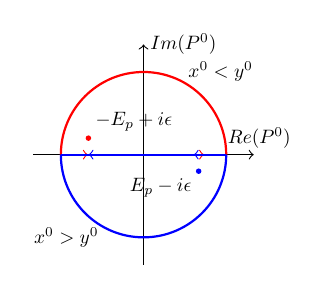
\begin{tikzpicture}[scale=.7]
        
      % Linea orizzontale (asse x)
       \draw[->] (-2,0) -- (2,0);
       \draw[->] (0,-2) -- (0,2)node[anchor=west,scale=.7]{$\mathfrak{Im} (P^0)$};

        % Semicirconferenza
        \draw[thick,red] (1.5,0) arc (0:180:1.5);
        \draw[>->,red] (-1.1,0) -- (1.1,0);
        \draw[thick,red] (-1.5,0) -- (1.5,0);

        \draw[thick,blue] (1.5,0) arc (0:-180:1.5);
        \draw[<-<,blue] (-1,0) -- (1,0);
        \draw[thick,blue] (-1.5,0) -- (1.5,0);

        \fill[blue,thick] (1,-0.3) circle  (.05)node[black,scale=0.7,anchor=north east]{$E_p-i\epsilon$};
        \fill[red,thick] (-1,0.3) circle  (.05)node[black,scale=0.7,anchor=south west]{$-E_p+i\epsilon$};
        
        \node[scale=.7] at (1.4,1.5) {$x^0<y^0$};
        \node[scale=.7] at (-1.4,-1.5) {$x^0>y^0$};
        \node[scale=.7] at (2.1,.3){$\mathfrak{Re} (P^0)$};

      \end{tikzpicture}
      \small Path used in the integration in the complex plane.
}
Using this prescription we can integrate in the complex plane with the poles translated by a bit up and down the real axis:
\begin{equation*}
    \Delta(x^\mu-y^\mu)=\int\frac{d^3p}{(2\pi)^3}e^{i\vec p\cdot \vec x}\bigg[\frac{e^{-iE_p\big(x^0-y^0\big)}}{2E_p}\theta\big(x^0-y^0\big)+\frac{e^{iE_p\big(x^0-y^0\big)}}{2E_p}\theta\big(y^0-x^0\big)\bigg],
\end{equation*}
where $\theta(x)$ is the Heaviside's step function, that is given by the fact that when $x^0>y^0$ Jordan's theorem wants the integration path to go in the lower part of the complex plane, thus we just have the contribution of the pole $z=E_p-i\epsilon$, and when $x^0<y^0$ we will have only the contribution of the other pole $z=-E_p+i\epsilon$.\\

Lastly we should concern about the interpretation of this result: since $y^0$ is the time at which the "point source" of the Green's function is located, the term resulting from $x^0>y^0$ should be interpreted as a particle going forward in time (from $y^0$ to $x^0$) and, as already anticipated, we can recognize that this has positive energy; the term resulting from $x^0<y^0$ should be interpreted as a particle going backwards in time and this has clearly a negative energy. 

